\documentclass[10pt,a4paper,roman, twocolumn]{article}  
%\documentclass[fontsize=10.5pt, twocolumn]{scrartcl}
\usepackage[a-1b]{pdfx}% formato PDF/A, obbligatorio per l'archiviazione delle tesi di Polito
\usepackage{amsmath}
\usepackage{amsfonts}
\usepackage{amssymb}
\usepackage{graphicx}
\usepackage[scale=0.85]{geometry}
\usepackage{color}
\usepackage{hyperref}
\usepackage{enumitem}


\usepackage[font=small,labelfont=bf]{caption}

\setlength{\parindent}{2em}
\setlength{\parskip}{0.2em}


\setlist[enumerate]{topsep=\parskip}
\setlist[itemize]{topsep=\parskip}

\hypersetup{%
	pdfpagemode={UseOutlines},
	bookmarksopen,
	pdfstartview={FitH},
	colorlinks,
	linkcolor={blue},
	citecolor={red},
	urlcolor={blue}
}

\title{\LARGE\textbf{Rethinking Automotive Software Development: Exploring Software Defined Vehicle and its potential}}
\author{
	\textbf{Candidate:} Lorenzo Sciara\\
	\textbf{Supervisors:} prof.~Danilo Bazzanella \\ dott.sa~Piera Limonet
}
\date{}



\begin{document}
\setlength{\belowdisplayskip}{0pt} \setlength{\belowdisplayshortskip}{0pt}
\setlength{\abovedisplayskip}{-0.5\baselineskip} \setlength{\abovedisplayshortskip}{-0.5\baselineskip}

	
\pagenumbering{gobble}
\maketitle
		
\section{Introduction and Motivation}
The \textit{Software Defined Vehicle} (SDV) paradigm is an innovative technology in the automotive industry that, by connecting the vehicle to cloud services and separating software development from supporting hardware systems, allows software to become a fundamental element of vehicle design. The resulting benefits are increased safety and efficiency of automobiles that can be remotely updated over their entire lifecycle using this innovation, and increased efficiency in the production of automotive software, reducing the waste of economic resources and development time. Additionally, this technology enables the activation or deactivation of vehicle features after the initial purchase, increasing the value of the vehicles and the company's revenue.

\subsection{Context}
In the context of the automotive industry, the software produced for vehicles was, until recently, always considered secondary to the production of the vehicles themselves. With the focus on the mechanical parts of the vehicle, software has been very dependent on the hardware for which it was implemented. The software production cycle for a new vehicle consisted of three phases. The development and testing phases were directly performed on the final hardware system. If the system responded correctly, the software was moved to the distribution phase for remaining more or less unchanged for the entire life of the car. Any modifications had to be made physically, resulting in significant resource waste. If the software did not respond correctly, the development and testing process had to be restarted on new hardware, resulting in additional costs and production delays.

The introduction of the SDV completely changes the paradigm. The vehicle's systems are no longer coordinated by special purpose devices related to the system itself, but rather by easily reprogrammable general purpose processors. Additionally, the vehicle is connected directly to the cloud for data analysis and the possibility of receiving \textit{Over The Air} (OTA) updates on any of its systems. At this point, the vehicle becomes a controllable device that can be easily updated based on the data and information it generates, similar to more common devices like smartphones or laptops. This increases both the production efficiency of the software and the safety of the vehicle, since any system vulnerability can be promptly identified, corrected and resolved through updates. Safety is a crucial aspect in the production of vehicle software, so much so that it is considered and classified by the \textit{International Organization for Standardization} (ISO) as a safety-critical device for human life.

In the last few years, several companies have come together to collaborate on the development of this technology. The Scalable Open Architecture for the Embedded Edge (SOAFEE) project was born from the cooperation of leading companies in the sector, including Amazon and Arm. Its goal is to create a software architectural standard based on Arm devices that can provide a cloud-native open-source environment for mixed-criticality automotive applications. The project is currently under development.

In view of the previous considerations, this thesis aims to provide an overview of the essential elements for creating the SDV and presents a practical project that illustrates its operation with the support of a Raspberry Pi board. The text begins with an overview of the state of the art technologies and approaches currently available, then moves to cloud computing and the advantages offered by \textit{Amazon Web Services} (AWS), and follows with an exploration of the use of AWS services in the context of the project. Finally, this document analyzes the implementation of the project in detail, describing all the development phases and illustrating the support tools used, such as \textit{Hawkbit} for deploying updates to the device and \textit{Grafana} for data analysis.

\section{Contributions of the thesis}
The thesis work's main contributions include defining a \textit{Telematics Control Unit} (TCU) simulator that can emulate the collection of data from vehicle subsystems. Additionally, a basic cloud infrastructure was built using AWS services to receive the telemetry data generated by the simulator and manage the development and deployment of updates on the device. The deployment server was implemented using \textit{Hawkbit}, a tool provided by \textit{Eclipse} that is specifically designed for deploying software to IoT devices. Additionally, a \textit{Grafana} server was implemented for data analysis. The proposed solution integrates elements from the state of the art further advance the field.

To make this solution effective, simplifications were made to the overall SDV concept to reduce complexity. All design and implementation decisions were made while considering the optimal trade-off between available resources and fidelity to the real use case.

The remainder of this section will present the contributions related to the construction phase of the cloud infrastructure -- Cloud Infrastructure -- as the simulator for collecting subsystem telemetry -- TCU Device Simulator -- as the data analysis server -- Grafana Server --. 

\subsection{Cloud Infrastructure}
The fundamental element of the proposed approach is the cloud infrastructure built through the use of the services offered by AWS. The architecture can be represented as two distinct workflows: one dedicated to the collection of telemetry data coming from the device, and the other to the management of the development and deployment of device update updates.

Regarding the data analysis flow illustrated in the figure \ref{fig:AWSDataServices}, a specific service for managing IoT devices is used, which is the IoT Core to collect data via a channel using the \textit{Message Queuing Telemetry Transport} (MQTT) protocol. The IoT Core service is also responsible for generating certificates to authenticate device connections. The data is then sent to a Kinesis stream, filtered by attributes and sent via a Lambda function to a Timestream database, which is in charge of temporarily storing the data.
\begin{figure} [tbh]
	\centerline{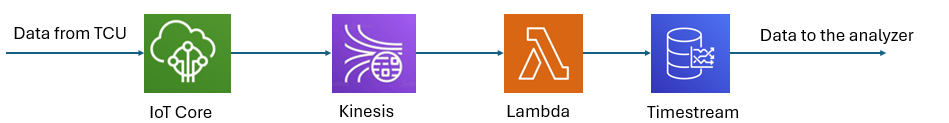
\includegraphics[width=0.4\textwidth]{images/AWS_data_services.png}}
	\caption{High-level representation of AWS services for data management}
	\label{fig:AWSDataServices}
\end{figure}

In terms of update management and deployment flow, the figure \ref{fig:AWSUpdateServices} shows the use of other services. First, an \textit{Elastic Compute Cloud} (EC2) instance is created in chronological order, on which the \textit{Hawkbit} server is installed. The server parameters, such as IP address and user information, are then saved in the \textit{System Manager}'s \textit{Parameter Store}. Subsequently, a pipeline is created, which consists of a \textit{Source} stage, a \textit{Build} stage, and a \textit{Deployment} stage, divided into three \textit{Lambda} functions, via the \textit{Codepipeline} service. The source stage uses a \textit{Codecommit} repository, which takes commit events to trigger subsequent actions in the pipeline. When an update of a compiled script written in C code, as in the project, is required, the repository containing the update source code is used as input by the build stage. This stage generates the executable file, which is ready for deployment from a specially created image placed in an \textit{Elastic Container Registry} (ECR) registry. At this point, the executable goes through the three Lambda functions that, by contacting the Hawkbit server with the information stored in the Parameter Store, respectively create the \textit{Distribution Set} and the \textit{Software Module} containing the update files on the server, create the \textit{Roll Out}, and assign the \textit{Distribution Set} to the device or fleet of devices to be updated, again using the API exposed by the \textit{Hawkbit} server.
\begin{figure} [tbh]
	\centerline{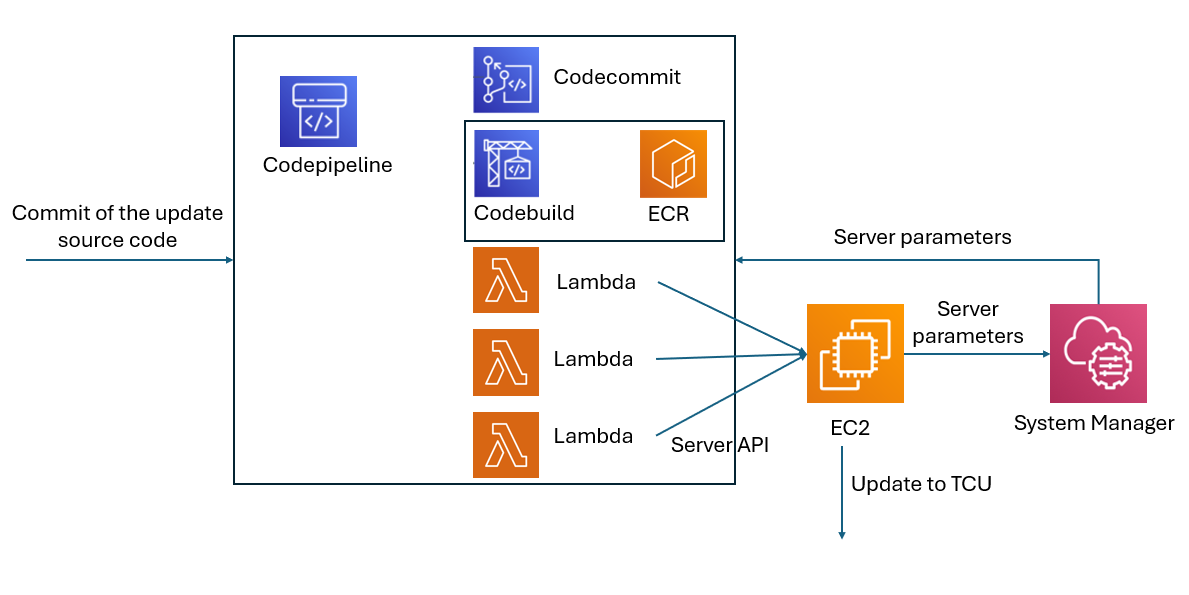
\includegraphics[width=0.4\textwidth]{images/AWS_update_services.png}}
	\caption{High-level representation of AWS services for the update management and deployment}
	\label{fig:AWSUpdateServices}
\end{figure}

These two execution flows in the cloud infrastructure appear to be separate, but they are linked by the device. The device receives updates and modifies performance and data produced, providing the necessary information to create new updates and continue this cycle throughout the device's life (and the potential vehicle's life). This passage demonstrates how the cloud services offered by AWS are a valid solution for the functions required for the development of the SDV.

\subsection{TCU Device Simulator}
The second essential element for the development of the thesis project is the TCU Device Simulator. It is a system that can collect and transmit data from simulated subsystems and integrate updates from external sources. The system is composed of four main elements:
\begin{enumerate}
	\setlength\itemsep{-0.3em}
	\item \textit{Data sender}, the component responsible for connecting to the cloud and sending the collected data;
	\item \textit{Update server connector}, the component responsible for connecting with the server that manages the deployment of updates;
	\item \textit{Data generator}, the component that collects data from the subsystems;
	\item \textit{Update agent}, the component that manages the activation of the update on the device.
\end{enumerate}

The four components working together enable the device simulator to generate, collect, and send data to the cloud infrastructure, as depicted in the image \ref{fig:TCUSimulatorP}. Additionally, the device remains in a constant state of readiness for any updates.
\begin{figure} [tbh]
	\centerline{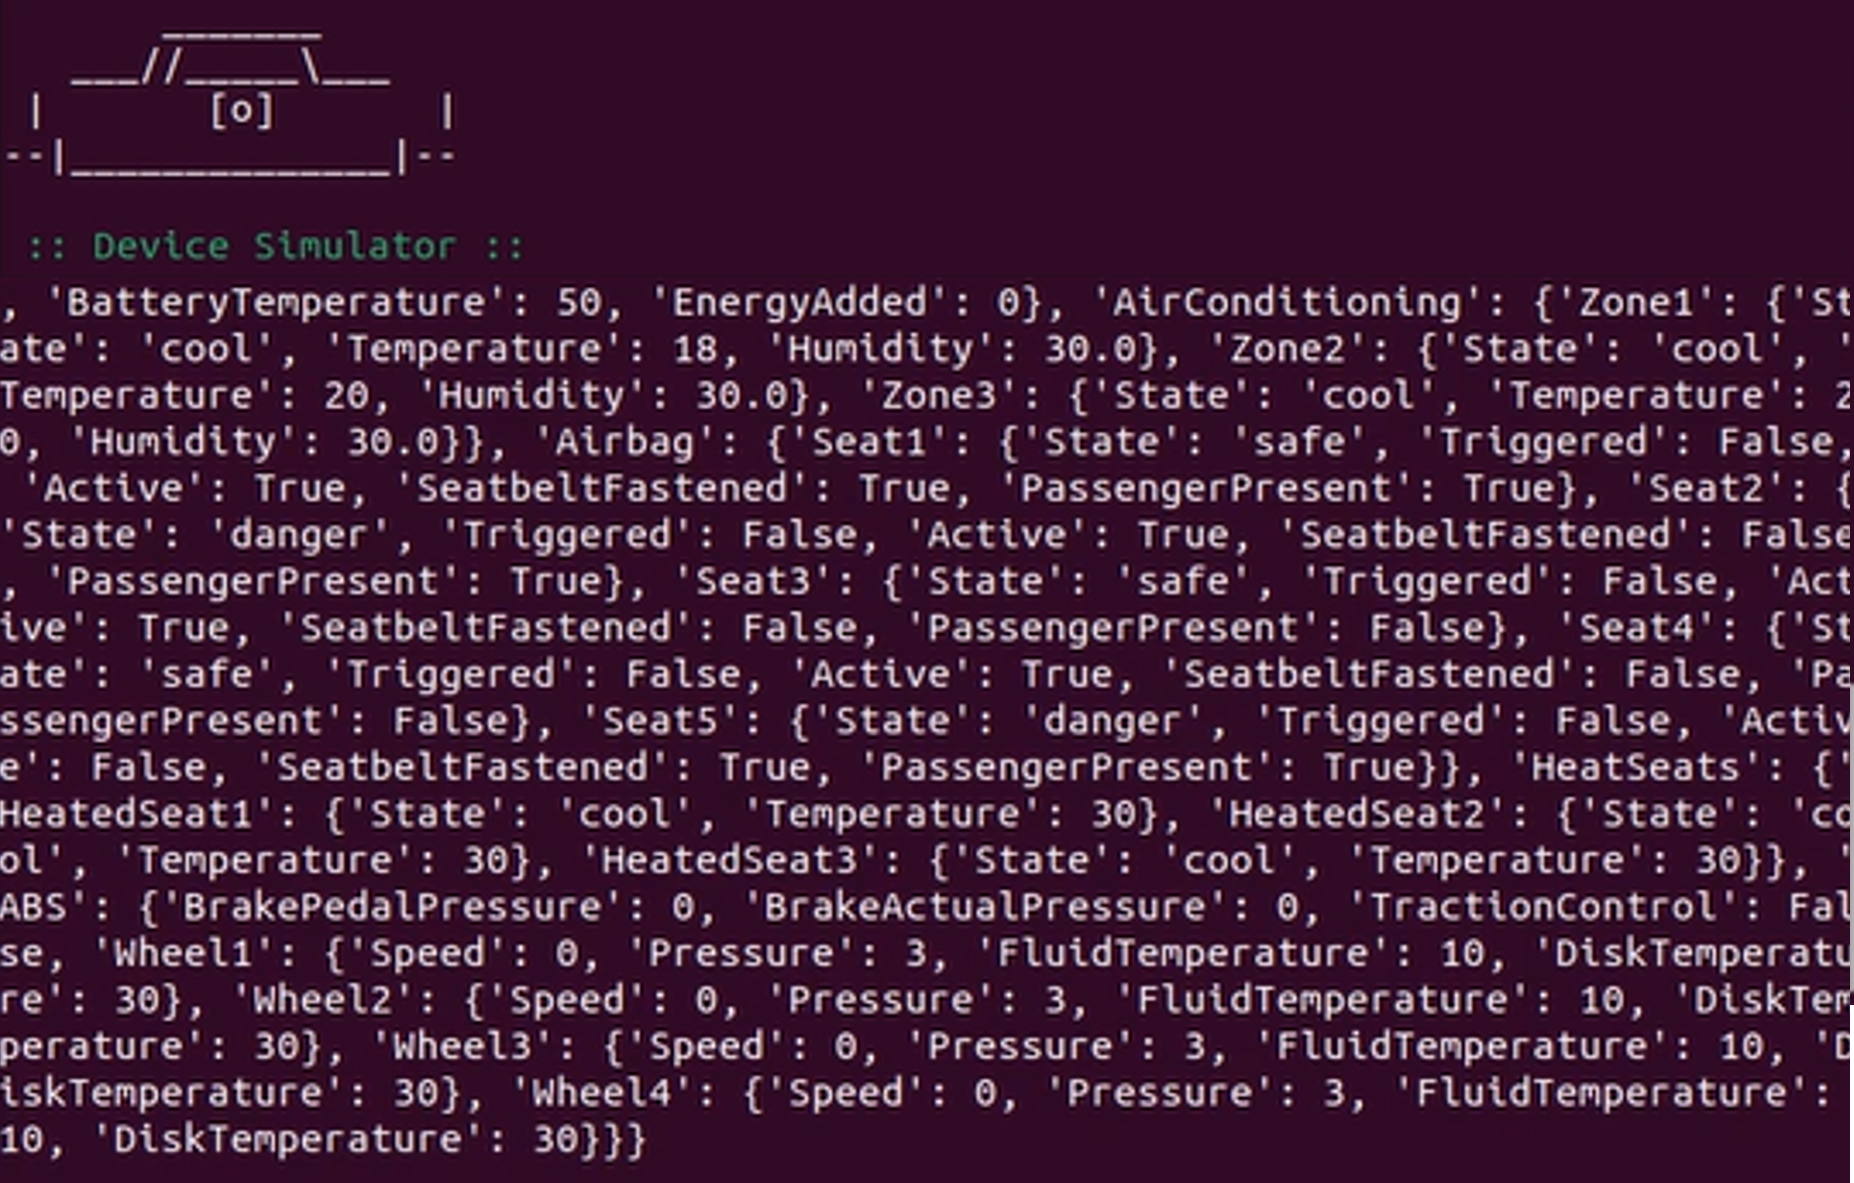
\includegraphics[width=0.3\textwidth]{images/TCUSimulatorP.png}}
	\caption{Snapshot of the TCU device simulator in action}
	\label{fig:TCUSimulatorP}
\end{figure}

This system enables the creation of a device simulator that can interact with the AWS services for data collection and storage, as well as with the Hawkibt server for deploying updates. The purpose of this simulator is to represent, in a simplified manner, the actions that would occur on a real vehicle in the context of SDV.

\subsection{Grafana Server}
The final component being analyzed is the data visualization feature using the Grafana server. Specifically, a docker image is utilized on a virtual machine to connect to the AWS Timestream database, retrieve real-time data, and display it to the user in easy to understand and intuitive dashboards.

This is done to provide a concrete representation of the generated data, making it easier to view and highlighting the update performed on the device simulator. In practice, the update in this example creates a variation in the data generated, similar to what would happen in a real case where an update on the vehicle's performance modifies its characteristics and the resulting data.
\begin{figure} [tbh]
	\centerline{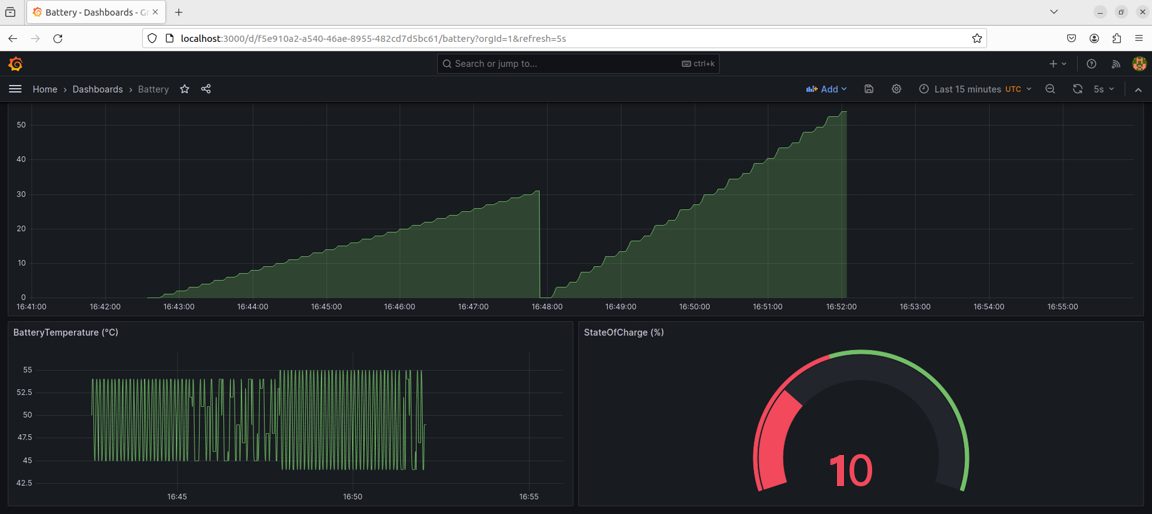
\includegraphics[width=0.4\textwidth]{images/grafana_Battery.png}}
	\caption{Snapshot of the Grafana battery dashboard of the device simulator in action}
	\label{fig:GrafanaBattery}
\end{figure}

Image \ref{fig:GrafanaBattery} displays a dashboard produced, highlighting the update on regenerative braking performance. The energy accumulated in the battery after the update is greater than before. However, the update also causes an increase in battery temperature peaks due to the increased performance and involvement of the subsystem in relation to the overall activities of the vehicle.

\section{PoC: Implementation and Validation}

The implementation of the framework has been made by exploiting the Java language, since the z3 theorem prover offers Java APIs to formulate and solve the MaxSMT problem. The interaction with the framework can be made through REST APIs, so that it can be exploited by external tools as a component of a more complex architecture.

This implementation has been, finally, tested extensively in common network scenarios and it showed good scalability against the dimension of the Service Graph and the number of input security requirements. The charts illustrated by Figure \ref{fig:perf01} and Figure \ref{fig:perf02} present the result of a series of tests performed to compare the scalability of the framework implementation related respectively to the number of Allocation Places and Network Security Requirements; in particular, the MaxSAT instances have been solved on a machine with Intel i7-6700 CPU running at 3.40 GHz and
32GB of RAM. 

The first information that can be extracted from the two charts is that the computation time does not increase exponentially either with the number of Allocation Places or with the number of NSRs; this is a very important result, given the computational complexity of the MaxSMT problem. Moreover, the framework scales to Service Graphs of medium-big dimensions, with a high number of links and end points, providing the optimal solution to the presented problem.

It is then possible to notice that an increment of the NSRs number produces a computation time higher than the one produced by the same increment of the Allocation Places number. This result is motivated by the fact that the verification of each requirement must be performed in all the network, considering packets that flow across all the possible paths, whereas the constraints introduced by an additional Allocation Place only impact the traffic flow which crosses that node.

\section{Conclusions and Future Work}
	 
This thesis demonstrates that the proposed approach is feasible and that it can provide a valid alternative in enforcing security functions to manual allocation and configuration of packet filtering firewalls, enabling low latency reaction to changes in security requirements. 

Furthermore, the approach has been developed to be compliant with future extensions such as the support of other NSFs in order to enrich its capabilities. Consequently, in the future the current methodology could be extended to the allocation and auto-configuration of other Network Security Functions, such as anti-spam filter, Web Application Firewall (WAF) and Intrusion Detection System (IDS). %, to further enrich the set of security requirements which can be specified by the user of the framework
Then, another possible future work is represented by the introduction of formal models for other network functions, such as the web cache, which the service designer can exploit to define the Service Graph.

%, on the other side definition of new Network Security Requirement types, which could consider additional features -- e.g. at application layer -- of the traffic flows to allow or to block. The goal would, in fact, be to further enrich the capabilities of the framework.

Finally, this thesis work represented the core content of a conference paper and a journal paper that will be submitted to IEEE/ACM Transactions on Networking in the next months.
	 
\end{document}

